% 编译方式：xelatex main_zh.tex && bibtex main_zh && xelatex main_zh.tex && xelatex main_zh.tex
\documentclass[UTF8]{ctexart}

\usepackage[margin=1in]{geometry}
\usepackage{microtype}
\usepackage{amsmath,amssymb,amsfonts}
\usepackage{array}
\usepackage{booktabs}
\usepackage[numbers]{natbib}
\usepackage{graphicx}
\usepackage{hyperref}
\usepackage{enumitem}
\usepackage{caption}

\setlist[itemize]{leftmargin=1.2em,itemsep=2pt,topsep=2pt}
\setlist[enumerate]{leftmargin=1.4em,itemsep=2pt,topsep=2pt}
\captionsetup{font=small,skip=4pt}
\setlength{\textfloatsep}{6pt plus 2pt minus 2pt}
\setlength{\floatsep}{6pt plus 2pt minus 2pt}
\setlength{\intextsep}{6pt plus 2pt minus 2pt}
\setlength{\abovecaptionskip}{4pt}
\setlength{\belowcaptionskip}{0pt}

\title{SREvoLab：面向符号回归的轻量级自动审查与演化框架}
\author{匿名作者}
\date{}

\begin{document}
\maketitle

\begin{abstract}
符号回归研究当前面临的主要瓶颈，越来越不只是方法本身，而是研究流程的工程碎片化。现有符号回归系统通常以彼此独立的仓库形式发布，在运行环境、执行假设、数据布局与表达式格式上互不兼容，从而难以在共享协议下完成复现、比较与扩展。本文提出 \textbf{SREvoLab}，一个面向符号回归的轻量级自动审查与演化框架。SREvoLab 目前已将 $10$ 个异构符号回归后端封装到统一执行接口之下，通过环境隔离管理处理依赖冲突，并将多类数据集标准化为轻量模式，包含 train/validation/ID-test/OOD-test 划分、元数据以及可选的真值公式。

在这一研究基底之上，我们进一步提供模块化技能，用于仓库接入、异构数据统一、协议编译、公式感知验证以及有边界的迭代改进。这些组件共同支持一个轻量的审查驱动闭环：系统首先对运行产物中的执行失败、协议风险和结果质量进行审查，再决定是否提出后续修改建议。我们将当前评估定位为基础设施验证，而非新的符号回归算法比较。具体而言，在标准化示例数据集上，公式验证可达到最低 $10^{-15}$ 量级的 split-level NMSE；与此同时，仓库中已归档的试点运行结果也能够在多种方法与数据集之间给出对齐的 ID/OOD 汇总。整体上，SREvoLab 为“先审查、后演化”的符号回归实验流程提供了一个可操作的基础。
\end{abstract}

\section{引言}

符号回归（symbolic regression, SR）旨在从数据中恢复紧凑、可解释的数学表达式，一直是科学机器学习与科学发现中的核心问题。当前的 SR 生态已经覆盖了早期面向科学发现的系统与物理启发式搜索方法 \citep{schmidt2009distilling,udrescu2020aifeynman,udrescu2020aifeynman2}，策略梯度与神经引导方法 \citep{petersen2021deep,mundhenk2021seeding}，预训练神经网络与 Transformer 型系统 \citep{biggio2021nsr,valipour2021symbolicgpt,kamienny2022end,vastl2022symformer,tpsr2023}，面向工程使用的软件栈如 PySR \citep{cranmer2023pysr}，以及近年来借助大语言模型的方案 \citep{shojaee2024llm,wang2025drsr}。然而，研究迭代速度受限的原因，往往并不亚于建模难度本身，而是工具链的高度碎片化。

一个典型的 SR 方法通常以独立仓库形式发布，附带各自不同的运行环境假设、数据约定、执行脚本和结果格式。不同 benchmark 家族之间还常常采用互不兼容的文件布局、数据划分规则、元数据组织方式、OOD 定义以及真值标注格式。因此，在真正开展科学比较之前，大量时间已经被消耗在仓库修复、环境隔离、数据重整、评测对齐和结果审计上。

本文的核心观点是：符号回归需要一个统一的\emph{研究基底}。这个基底应当能够让异构方法在共享协议下运行，让异构数据集在共享模式下被消费，并将整个流程暴露给结构化自动化机制。基于这一目标，我们提出 \textbf{SREvoLab}，一个面向符号回归的轻量级自动审查与演化框架，用于降低方法接入、数据标准化、可复现实验执行以及有边界迭代改进的成本。图~\ref{fig:problem-definition-overview} 概括了本文的问题背景与主要贡献。

\begin{figure}[t]
    \centering
    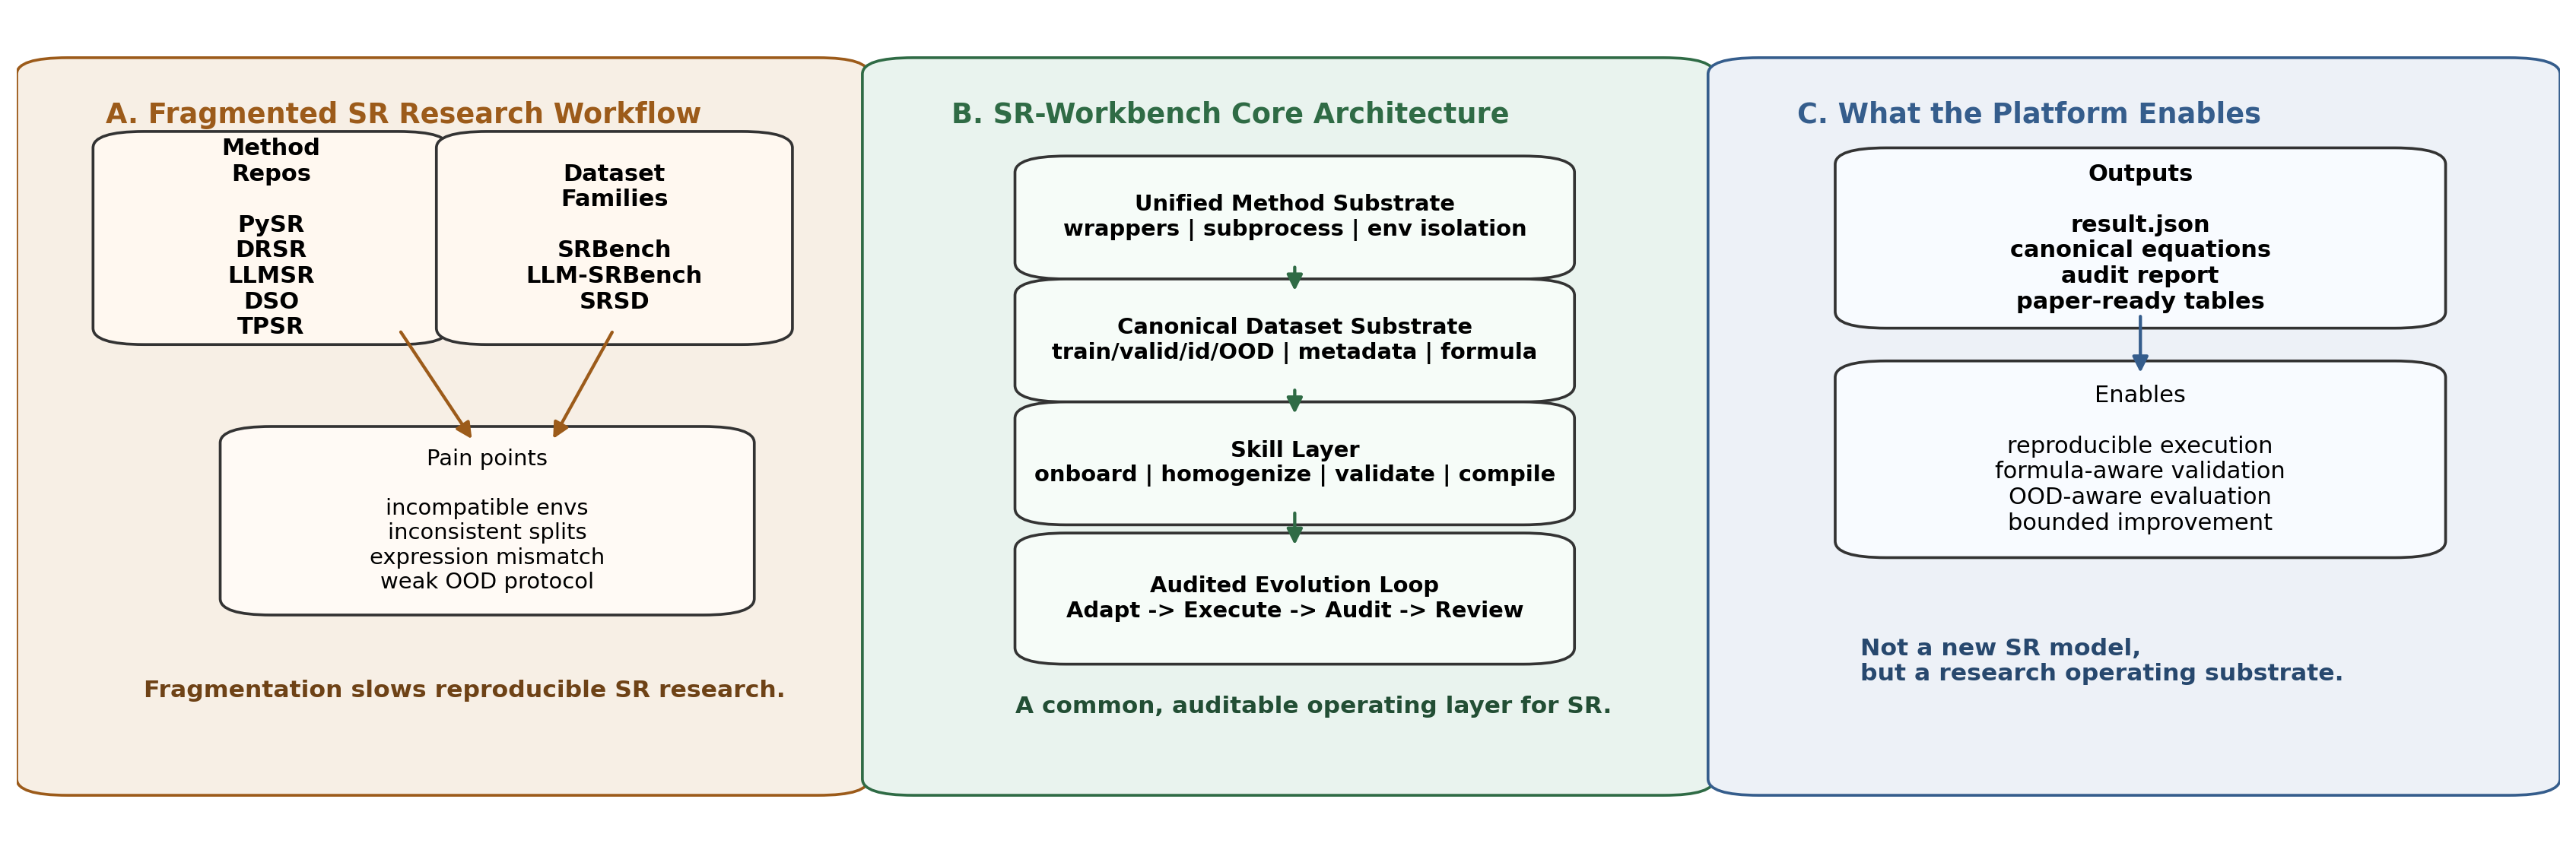
\includegraphics[width=\linewidth]{figures/problem_definition_contributions_figure.png}
    \caption{从碎片化的符号回归仓库与异构 benchmark 格式，到统一、可审计的研究基底。SREvoLab 对方法执行、数据结构与高频研究操作进行标准化，并在其上叠加一个轻量的审查驱动演化闭环。本文的核心贡献不是提出新的符号回归模型，而是构建一个可以降低工程熵、支持可复现且可扩展 SR 实验的研究操作层。}
    \label{fig:problem-definition-overview}
\end{figure}

SREvoLab 建立在两层标准化机制之上。第一层是\emph{统一方法接口}：代表性的 SR 系统被封装在统一执行契约之后，对外暴露训练、预测与公式提取能力，同时通过环境管理隔离不兼容依赖。当前平台已经整合了十个异构 SR 后端，覆盖经典方法、搜索型方法和 LLM 辅助方法。第二层是\emph{规范化数据集模式}：将 SRBench、LLM-SRBench 与 SRSD 风格的数据源重组为轻量统一格式，包含 \texttt{train.csv}、\texttt{valid.csv}、\texttt{id\_test.csv}、\texttt{ood\_test.csv}、\texttt{metadata.yaml} 以及可选的真值公式文件。

在这两层基底之上，我们进一步引入模块化的\emph{技能层}。SREvoLab 不再将仓库集成、数据转换、协议检查和表达式处理视为零散的临时杂务，而是把它们包装成可复用操作，例如仓库接入、异构数据标准化、表达式归一化以及公式真值验证。

最后，我们给出一个轻量的\emph{审查驱动演化闭环}。这一闭环从一个可运行基线出发，先编译保持协议不变的实验规格，再执行运行、审查产物，最后才提出受约束的后续修改建议。其重点并不是无限制的自动搜索，而是在固定 benchmark 语义下开展纪律化迭代。这里最关键的设计原则是\emph{先审查、后演化}：演化的驱动力来自对日志、公式、指标与审计标记的结构化反馈，而不是不受控制的分数追逐。当前稿件用三个具体资产支撑这一主张：一个覆盖 $10$ 个工具、$8$ 个环境的方法基底；在标准化数据集上最低达到 $10^{-15}$ NMSE 的公式验证；以及能够在统一结果格式下呈现显著 ID/OOD 差异的试点结果切片。

本文的主要贡献如下：
\begin{itemize}[leftmargin=1.5em]
    \item 我们构建了一个统一的符号回归研究基底，在一个封装接口下整合了十个异构 SR 工具，并通过八个受控执行环境完成依赖隔离。
    \item 我们提出了一种轻量的数据集规范化模式，显式包含 train/validation/ID-test/OOD-test 划分、元数据与可选真值公式，并在存在解析表达式时进行数值一致性验证。
    \item 我们实现了一个面向仓库接入、数据同构化与公式感知验证的模块化技能层，将高频 SR 工程工作显式化、复用化。
    \item 我们提出了一个审查优先的演化闭环，将运行产物映射为有边界的下一步动作建议，同时保持 benchmark 语义与评测完整性不被破坏。
\end{itemize}

\section{相关工作}

\paragraph{符号回归基准评测。}
符号回归社区已经多次指出，科学进展不仅受算法限制，也受到基准评测纪律不足的约束。SRBench \citep{lacava2021srbench} 构建了一个可复现的比较流程，用于在真实问题与具备真值公式的问题之间开展统一评测；随后的工作进一步讨论了超参数调优、执行约束与 benchmark 维护问题 \citep{aldeia2025call}。本文与这条研究路线在目标上是一致的，但关注层次不同：我们并不只是扩展 benchmark，而是试图构建一个运行基底，使异构方法与异构数据集能够在共享协议下真正运行起来。

\paragraph{面向科学符号回归的数据集。}
数据集设计已经成为符号回归研究中的核心议题。SRSD \citep{matsubara2022rethinking} 指出许多现有数据集并不适合科学发现语境，并提出了更贴近真实场景的公式采样范围以及树结构感知的公式比较策略。LLM-SRBench \citep{shojaee2025llmsrbench} 则进一步强调了数据划分设计和公式感知评测对大语言模型系统的重要性。SREvoLab 沿着这一方向推进，但重点放在把多个 benchmark 家族统一整理为同一种模式，显式提供 validation、ID-test、OOD-test、元数据以及可选的公式验证入口。

\paragraph{统一或混合式符号回归框架。}
已有若干工作尝试在算法层面对符号回归能力进行统一。较早的代表包括基于符号回归的定律发现系统 \citep{schmidt2009distilling} 和面向物理问题的递归分解方法 \citep{udrescu2020aifeynman,udrescu2020aifeynman2}。更新的方法覆盖风险偏好的策略梯度搜索 \citep{petersen2021deep}、神经引导的种群初始化 \citep{mundhenk2021seeding}、大规模预训练 \citep{biggio2021nsr}、基于 Transformer 的端到端生成 \citep{valipour2021symbolicgpt,kamienny2022end,vastl2022symformer,tpsr2023}、工程化软件栈 \citep{cranmer2023pysr} 以及近期的 LLM 辅助方程发现方法 \citep{shojaee2024llm,wang2025drsr}。其中具有代表性的统一框架是 uDSR \citep{landajuela2022udsr}，它在一个模块化模型家族中整合了多种求解策略。与这些工作不同，本文的目标不是统一建模家族，而是统一那些原本彼此独立维护、从未被设计为可共存的仓库、环境、数据集与执行语义。

\paragraph{自动化科研基础设施。}
近年来，自动化科研系统开始尝试将论文、代码仓库与实验流程组织为部分自动化的优化闭环。在更广义的机器学习系统层面，可复现性倡议也持续强调清单化报告与可执行科研工作流的重要性 \citep{pineau2021improving}。例如，AutoSOTA \citep{li2026autosota} 贯穿了论文理解、环境修复、实验执行、创新生成与有效性监督等多个环节。SREvoLab 与这一基础设施视角相呼应，但刻意保持轻量且领域专用：它面向符号回归的特定需求，例如公式输出、复杂度敏感评估、OOD 报告以及可选真值验证。换言之，它处在“更好的 SR benchmark”和“更通用的自动化科研系统”之间，专注于一个更具体、更可落地的中间层。

\section{系统概览与方法}

\subsection{问题设定与设计目标}

SREvoLab 面向这样一个现实研究场景：符号回归的进展经常不是被方法创新本身阻碍，而是被异构仓库、异构数据集与不一致的执行协议所拖慢。我们的目标不是用一个统一模型替换现有 SR 方法，而是提供一个公共操作层，使这些方法能够以更低的接入成本被复现、比较和扩展。基于这一目标，我们提出四项设计原则：
\begin{enumerate}[leftmargin=1.5em]
    \item \textbf{方法层统一：}异构符号回归仓库应当暴露共享的训练、预测与公式提取接口。
    \item \textbf{数据层统一：}异构 benchmark 家族应当被转换为共享模式，并显式支持 validation 与 OOD 评测槽位。
    \item \textbf{操作模块化：}高频研究操作应当被上浮为可复用技能，而不是继续停留在零散的手工步骤中。
    \item \textbf{协议保持：}任何迭代改进机制都必须遵守固定的 benchmark 语义、数据划分使用规则与评测流程。
\end{enumerate}

从整体架构上看，SREvoLab 由方法基底、数据基底、技能层以及轻量审查驱动演化闭环组成。其控制原则很简单：每一次运行都必须先被解释和审查，之后才能进入后续改动阶段。

\subsection{统一方法基底}

SREvoLab 的核心入口是统一方法接口 \texttt{SymbolicRegressor}。每个后端都被封装为工具适配器，实现四个主要操作：\texttt{fit}、\texttt{predict}、\texttt{get\_optimal\_equation} 和 \texttt{get\_total\_equations}。这些适配器负责隐藏工具特定的细节，例如仓库布局、模型初始化、表达式提取约定与序列化方式。

方法注册采用配置驱动方式。工具注册表将每个工具标识映射到具体 wrapper 类和隔离运行环境。当前注册表已经覆盖十个异构后端，包括工程软件导向的 PySR \citep{cranmer2023pysr}、与 DSO/uDSR 相关的强化学习和神经引导方法 \citep{petersen2021deep,mundhenk2021seeding,landajuela2022udsr}、NeSymReS/E2E/TPSR 等 Transformer 家族 \citep{biggio2021nsr,kamienny2022end,tpsr2023}，以及近期的 LLM 辅助系统 \citep{shojaee2024llm,wang2025drsr}。表~\ref{tab:method-coverage} 给出了当前方法基底的覆盖情况。

\begin{table}[t]
\centering
\scriptsize
\begin{tabular}{llll}
\toprule
方法 & Wrapper 类 & 环境 & 注册状态 \\
\midrule
\texttt{QLattice} & \texttt{QLatticeRegressor} & \texttt{sim\_qLattice} & 已集成 \\
\texttt{drsr} & \texttt{DRSRRegressor} & \texttt{sim\_llm} & 已集成 \\
\texttt{dso} & \texttt{DSORegressor} & \texttt{sim\_dso} & 已集成 \\
\texttt{e2esr} & \texttt{E2ESRRegressor} & \texttt{sim\_e2esr} & 已集成 \\
\texttt{gplearn} & \texttt{GPLearnRegressor} & \texttt{sim\_base} & 已集成 \\
\texttt{iMCTS} & \texttt{iMCTSRegressor} & \texttt{sim\_iMCTS} & 已集成 \\
\texttt{llmsr} & \texttt{LLMSRRegressor} & \texttt{sim\_llm} & 已集成 \\
\texttt{pyoperon} & \texttt{OperonRegressor} & \texttt{sim\_base} & 已集成 \\
\texttt{pysr} & \texttt{PySRRegressor} & \texttt{sim\_base} & 已集成 \\
\texttt{tpsr} & \texttt{TPSRRegressor} & \texttt{sim\_tpsr} & 已集成 \\
\bottomrule
\end{tabular}
\caption{SREvoLab 当前方法注册表的覆盖范围。每个工具都通过共享符号回归接口暴露，并映射到受控执行环境。}
\label{tab:method-coverage}
\end{table}

系统通过子进程边界执行具体方法。SREvoLab 将动作类型、数据载荷、工具标识与运行参数序列化后，分发给工具专属的子进程执行器。这一设计能够隔离异构 SR 栈之间的依赖冲突，并通过将后端崩溃与编排层解耦来提升整体鲁棒性。每次运行还会记录最小实验元数据，例如工具名、任务名、随机种子、配置与执行状态。

每个后端都绑定一个专用或共享的 conda 环境，使平台能够同时支持依赖 Python 版本不同或第三方库冲突严重的多类工具。

\subsection{规范化数据基底}

数据基底将异构 SR benchmark 转换为统一的目录式模式：
\begin{center}
\texttt{train.csv, valid.csv, id\_test.csv, ood\_test.csv, metadata.yaml, formula.py (optional)}.
\end{center}
所有 CSV 文件都必须共享一致的表头，元数据则提供目标列名、特征名、划分信息以及可选语义描述。表~\ref{tab:dataset-schema} 总结了该模式。

\begin{table}[t]
\centering
\scriptsize
\begin{tabular}{>{\raggedright\arraybackslash}p{2.4cm}>{\raggedright\arraybackslash}p{1.4cm}>{\raggedright\arraybackslash}p{3.0cm}>{\raggedright\arraybackslash}p{4.1cm}}
\toprule
工件 & 必需 & 角色 & 验证内容 \\
\midrule
\texttt{train.csv} & 是 & 训练划分 & 表头、样本行、目标列 \\
\texttt{valid.csv} & 是 & 模型选择划分 & 表头、样本行、目标列 \\
\texttt{id\_test.csv} & 是 & 分布内测试 & 表头、样本行、目标列 \\
\texttt{ood\_test.csv} & 是 & 分布外测试 & 表头、样本行、目标列 \\
\texttt{metadata.yaml} & 是 & 目标/特征/划分元信息 & 结构与计数一致性 \\
\texttt{formula.py} & 否 & 解析真值公式 & 可调用性与数值匹配 \\
\bottomrule
\end{tabular}
\caption{SREvoLab 使用的规范化数据集模式。验证器会检查数据划分一致性，并在存在解析公式时执行额外的真值验证。}
\label{tab:dataset-schema}
\end{table}

这一模式针对 SR 实验中的三类常见摩擦点给出了解法：它移除了仓库特定的文件命名与划分布局假设，使 OOD 评测成为显式结构，并为数据集级语义信息提供稳定位置。

当数据集提供真值公式时，SREvoLab 会显式保存该公式，并对其进行验证，而不是把它当成被动注释。当前验证器会导入声明的公式、按照元数据中记录的特征顺序对齐其参数签名，并检查公式计算结果与目标列在数值容差内的一致性。真值公式因此被视为验证工件，而不是搜索过程中的特权信息。

\subsection{技能层}

SREvoLab 将高频研究操作上浮为显式技能。在当前系统中，两个 SR 专用技能构成主要操作骨架。

第一个技能 \texttt{sr-tool-onboarder} 用于标准化接入新的符号回归仓库，覆盖 manifest 管理、wrapper 脚手架生成、环境注册以及运行时验证。

第二个技能 \texttt{heterogeneous-data-to-examples} 用于将异构源数据统一转换为规范化数据集模式，包括带划分的数据集目录、元数据模板与公式感知验证流程。

从操作层面看，技能层降低了重复性工程成本，也使整体工作流足够显式，从而可以被审计并进一步自动化。

\subsection{轻量审查驱动演化闭环}

在统一的方法基底与数据基底之上，我们定义了一个轻量的审查驱动演化闭环。它追求的是有边界、保持协议的迭代，而不是无约束的自动优化。其标准轨迹可以写为：
\begin{center}
\texttt{Adapt $\rightarrow$ Compile $\rightarrow$ Execute $\rightarrow$ Normalize $\rightarrow$ Audit $\rightarrow$ Review $\rightarrow$ Archive}.
\end{center}

\paragraph{Adapt（适配）。}
从一个候选符号回归仓库出发，系统先通过统一 wrapper 接口完成方法接入，并记录其可执行配置。

\paragraph{Compile（编译协议）。}
给定一个规范化数据集和一份方法配置，系统生成实验规格，固定工具、数据集、参数包、随机种子与评测目标。在这一步，benchmark 语义被冻结。

\paragraph{Execute（执行）。}
系统在统一执行基底下运行配置好的后端，得到一个可复现的产物包，其中包含日志、公式输出、运行元数据以及评测汇总。

\paragraph{Normalize（归一化）。}
方法输出会被映射到共享表示中，包括公式字符串以及在可用时给出的候选公式集合。该步骤也是后续表达式化简或常数精修的潜在插入点。

\paragraph{Audit（审查）。}
在接受任何性能改进结论之前，闭环都会先执行显式有效性检查。审查层旨在阻止 benchmark 漂移与协议违规，包括修改评测脚本、悄然重定义数据划分、使用不一致指标以及把真值公式泄露到搜索过程中。一旦审查失败，演化动作不得继续。

\paragraph{Review and Archive（复盘与归档）。}
最后，系统总结该次运行，记录失败模式或候选改进方向，并将产物状态归档，供后续继续迭代。更具体地说，复盘器会把一次运行映射到一个小型动作词表中：保留当前基线、修复执行问题、调整受约束超参数，或尝试结构层改动，例如替换算子集合或添加后处理步骤。任何改变评测语义、数据划分定义或把真值泄露给搜索过程的动作都被明确禁止。因此，当前实现更应被理解为“以审查为门控的轻量迭代脚手架”，而不是一个完整的自主科研代理。

\section{实验}

\subsection{实验范围}

由于 SREvoLab 的定位是研究基底而非新的符号回归算法，实验主要验证三个性质：方法覆盖能力、数据模式有效性以及在可控试点切片上的端到端执行能力。因此，我们不把当前结果解读为最终 leaderboard 结论。更准确地说，这一版本验证的是自动审查与受约束演化所需的基础设施是否已经具备。

更具体地，实验围绕三个主张展开。\textbf{C1}：异构 SR 方法能够在共享操作层下被执行。\textbf{C2}：异构数据集能够被标准化为一种统一模式，并保持可验证的数据划分与公式语义。\textbf{C3}：当方法与数据都被归一化后，系统能够产出对齐的 ID/OOD 行为报告，为后续的审查驱动演化提供输入。

在方法层面，当前注册表整合了 $10$ 个符号回归工具，并映射到 $8$ 个 conda 环境，这反映出 SR 仓库之间确实存在显著的依赖栈不兼容问题。

\subsection{数据模式与公式验证}

我们首先验证规范化数据基底本身。当前 examples 风格的模式要求四个对齐的数据划分文件、一个 \texttt{metadata.yaml}，以及在存在解析真值时可选的 \texttt{formula.py}。验证脚本会检查划分文件是否完整、表头是否一致、目标列与特征列是否匹配、声明样本数是否正确，以及在可用时进一步检查公式一致性。

对于具有已知解析公式的数据集，验证器会导入声明的公式函数，按照元数据中记录的特征顺序对齐其参数，并将公式输出与目标列进行比较。作为一致性检查，当前实现验证了 examples 目录下 \texttt{BPG0} 与 \texttt{BPG1} 的真值公式。在 \texttt{BPG0} 上，公式检查在 train/validation/ID 数据上的 split-level NMSE 约为 $10^{-13}$，在 OOD 数据上约为 $10^{-9}$；在 \texttt{BPG1} 上，对应 NMSE 则达到约 $10^{-15}$。这直接支撑了 \textbf{C2}：该模式不只是保存元数据和公式，更保留了可数值检查的语义一致性。

\subsection{端到端试点切片}

为了评估平台的可执行性，我们进一步汇报一个覆盖三个代表性数据集的试点切片：\texttt{oscillator1}、\texttt{oscillator2} 和 \texttt{stressstrain}。我们选取了三个已经在 SREvoLab 中具备稳定端到端执行路径的方法：\texttt{pysr}、\texttt{llmsr} 和 \texttt{drsr}。表中的结果来自仓库中通过统一执行路径生成并归档的 \texttt{result.json} 文件。

这些运行结果应被理解为\emph{研究基底验证案例}，而非最终 benchmark 比较。它们的目的在于说明：平台已经能够在规范化数据集上运行多个异构方法，并给出对齐的 ID/OOD 汇总。

表~\ref{tab:pilot-slice} 汇总了当前试点结果。已经可以看到三个明显现象：第一，平台可以在统一结果结构下同时报告 ID 与 OOD 行为；第二，在 oscillator 任务上，OOD 行为比 ID 行为更能区分方法差异；第三，LLM 辅助方法与经典方法现在已经可以在同一执行基底内被直接比较。结合前文的方法注册统计，这些结果共同支撑了 \textbf{C1} 与 \textbf{C3}。

\begin{table}[t]
\centering
\scriptsize
\begin{tabular}{llrrrr}
\toprule
方法 & 数据集 & ID RMSE & OOD RMSE & ID NMSE & OOD NMSE \\
\midrule
\texttt{drsr} & \texttt{oscillator1} & $3.54\times 10^{-6}$ & $3.94\times 10^{-3}$ & $2.75\times 10^{-9}$ & $2.03\times 10^{-3}$ \\
\texttt{drsr} & \texttt{oscillator2} & $8.34\times 10^{-6}$ & $1.13\times 10^{-3}$ & $4.24\times 10^{-10}$ & $1.33\times 10^{-6}$ \\
\texttt{drsr} & \texttt{stressstrain} & $4.81\times 10^{-2}$ & $4.01\times 10^{-2}$ & $5.93\times 10^{-3}$ & $5.49\times 10^{-3}$ \\
\texttt{llmsr} & \texttt{oscillator1} & $7.01\times 10^{-4}$ & $2.75\times 10^{-2}$ & $1.08\times 10^{-4}$ & $9.91\times 10^{-2}$ \\
\texttt{llmsr} & \texttt{oscillator2} & $1.19\times 10^{-3}$ & $3.40\times 10^{-2}$ & $8.62\times 10^{-6}$ & $1.19\times 10^{-3}$ \\
\texttt{llmsr} & \texttt{stressstrain} & $5.56\times 10^{-2}$ & $4.99\times 10^{-2}$ & $7.90\times 10^{-3}$ & $8.51\times 10^{-3}$ \\
\texttt{pysr} & \texttt{oscillator1} & $1.99\times 10^{-3}$ & $6.17\times 10^{-2}$ & $8.68\times 10^{-4}$ & $4.97\times 10^{-1}$ \\
\texttt{pysr} & \texttt{oscillator2} & $1.55\times 10^{-1}$ & $1.11$ & $1.46\times 10^{-1}$ & $1.28$ \\
\texttt{pysr} & \texttt{stressstrain} & $5.23\times 10^{-2}$ & $4.88\times 10^{-2}$ & $7.00\times 10^{-3}$ & $8.13\times 10^{-3}$ \\
\bottomrule
\end{tabular}
\caption{通过 SREvoLab 统一执行路径运行并归档的试点结果。当前表格用于系统能力验证，而不是最终排行榜结论。}
\label{tab:pilot-slice}
\end{table}

这个试点切片还说明了为什么一个带审查机制的研究基底是有价值的。在某些任务上，尤其是 \texttt{oscillator2}，ID 与 OOD 行为之间的差距足够大，以至于只看 ID 指标会得出误导性结论。例如，\texttt{drsr} 在该任务上取得了 $1.33\times 10^{-6}$ 的 OOD NMSE，而 \texttt{pysr} 则上升到 $1.28$。相比之下，在 \texttt{stressstrain} 上，三种方法的 OOD NMSE 都落在大约 $5\times 10^{-3}$ 到 $9\times 10^{-3}$ 的窄区间内，这提示后续比较不能只看预测误差，还应纳入复杂度与稳定性。这恰恰是审查模块在提出下一步受约束改动之前应当重点消费的证据。

\subsection{当前评估的局限性}

当前实验刻意保持在较窄范围内。试点切片只覆盖了部分已集成方法和任务，尚未在所有后端上实施统一冻结的跨方法计算预算，也还没有充分利用表达式级归一化与复杂度感知排序。完整的闭环自动审查与演化研究仍然属于下一阶段工作。因此，我们将当前实验视为“平台已经可用”的证明，而接下来的重点则是扩展协议覆盖面并进一步强化公平性保证。

\section{结论}

本文提出了 SREvoLab，一个统一的符号回归研究平台，用于在同一研究基底下标准化异构方法、异构数据集以及高频研究操作。与其说我们提出了又一个符号回归模型，不如说我们直接针对 SR 研究中最常见的基础设施瓶颈：仓库碎片化、环境不兼容、数据约定不一致以及协议控制薄弱。

当前版本已经展示了三项实用能力：第一，将多类 SR 方法接入统一执行接口；第二，在数据模式层面提供包括真值公式验证在内的标准化校验；第三，在共享结果格式下完成端到端试点运行，并同时暴露 ID 与 OOD 行为。这三项能力与论文的核心主张一一对应，也使得当前贡献不只是若干软件 wrapper 的堆叠。

与此同时，我们有意将本文视为系统的第一版发布，而非最终 benchmark 结论。下一阶段需要进一步强化固定预算下的跨方法公平比较、表达式归一化与复杂度分析、协议编译机制以及审查驱动的改进调度。最重要的下一步，是在更广的 benchmark 切片上验证完整的“先审查、后演化”闭环。

更广义地看，符号回归的进步往往不仅受搜索算法本身限制，也受制于缺乏可靠研究基础设施。通过把方法接入、数据标准化、验证、审查与迭代执行变成显式且可复用的操作，SREvoLab 朝着更快、更可复现、更可扩展的 SR 研究流程迈出了一步。

\bibliographystyle{plainnat}
\bibliography{references}

\end{document}
